\documentclass{neu_handout}
\usepackage{url}
\usepackage{amssymb}
\usepackage{amsmath}
\usepackage{marvosym}
\usepackage{graphicx}
\usepackage[pdftex]{graphicx}
\usepackage{subfigure}
\graphicspath{ {images/} }
\everymath{\displaystyle}

% Professor/Course information
\title{Homework 0}
\author{Emily Dutile}
\date{January 2018}
\course{CS 7295}{Information Visualization}

\begin{document}

\begin{figure}[h]
\centering
{
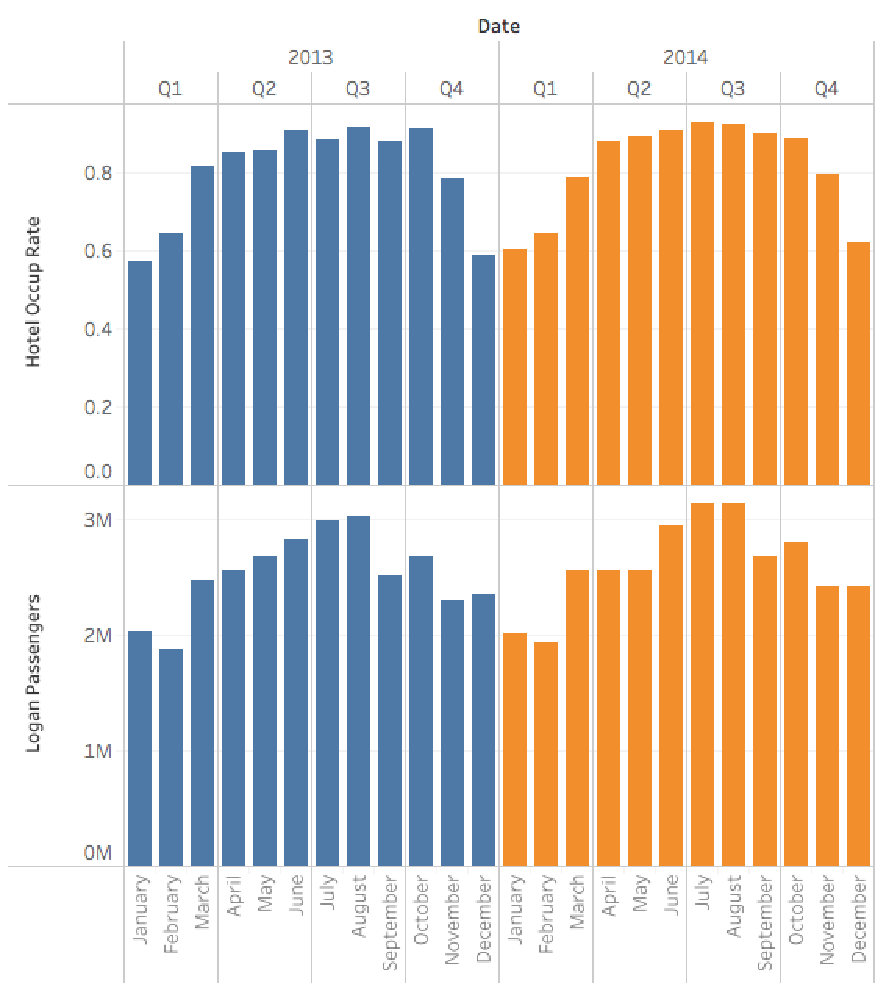
\includegraphics[width=0.4\linewidth]{tableau}
}
\end{figure}

I was curious to see a trend with respect to the hotel occupancy rate and the season. My hypothesis was that more people tend to travel in the summer months due to nicer weather and school vacation, so I would expect there to be an increase in hotel occupancy. This would be insightful for business owners in order to know when to increase prices due to demand. This chart shows a huge drop off in winter months (December-February) and seems to be consistent in both years. The charts align with my original thoughts.

\end{document}
